\documentclass[
  captions=tableheading,
  bibliography=totoc, 
  titepage=firstiscover,
]{scrartcl}

\usepackage{blindtext} %neuer input

\usepackage{longtable} % Tabellen über mehrere Seiten

\usepackage[utf8]{inputenc} %neuer input

\usepackage{scrhack}

\usepackage[aux]{rerunfilecheck} %Warnung falls nochmal kompiliert werden muss

\usepackage{fontspec} %Fonteinstellungen

\recalctypearea{}

\usepackage[main=ngerman]{babel} %deutsche Spracheinstellung

\usepackage{ragged2e} %neuer input

\usepackage{amsmath, nccmath}

\usepackage{amssymb} %viele mathe Symbole

\usepackage{mathtools} %Erweiterungen für amsmath


\DeclarePairedDelimiter{\abs}{\lvert}{\rvert}
\DeclarePairedDelimiter{\norm}{\lVert}{\rVert}

\DeclarePairedDelimiter{\bra}{\langle}{\rvert}
\DeclarePairedDelimiter{\ket}{\lvert}{\rangle}

\DeclarePairedDelimiterX{\braket}[2]{\langle}{\rangle}{
#1 \delimsize| #2
}

\NewDocumentCommand \dif {m}
{
\mathinner{\symup{d} #1}
}


\usepackage[
  math-style=ISO,
  bold-style=ISO,
  sans-style=italic,
  nabla=upright,
  partial=upright,
  warnings-off={
    mathtools-colon,
    mathtools-overbracket,
  },
]{unicode-math}

\setmathfont{Latin Modern Math}
\setmathfont{XITS Math}[range={scr, bfscr}]
\setmathfont{XITS Math}[range={cal, bfcal}, StylisticSet=1]


\usepackage[
  locale=DE,
  separate-uncertainty=true,
  per-mode=reciprocal,
  output-decimal-marker={,},
]{siunitx}

\usepackage[autostyle]{csquotes} %richtige Anführungszeichen

\usepackage{xfrac}

\usepackage{float}

\floatplacement{figure}{htbp}

\floatplacement{table}{htbp}

\usepackage[ %floats innerhalb einer section halten
  section,   %floats innerhalb er section halten
  below,     %unterhalb der Section aber auf der selben Seite ist ok
]{placeins}

\usepackage[
  labelfont=bf,
  font=small,
  width=0.9\textwidth,
]{caption}

\usepackage{subcaption} %subfigure, subtable, subref

\usepackage{graphicx}

\usepackage{grffile}

\usepackage{booktabs}

\usepackage{microtype} %Verbesserungen am Schriftbild

\usepackage[
backend=biber,
]{biblatex}

\addbibresource{../lit.bib}

\usepackage[ %Hyperlinks im Dokument
  german,
  unicode,
  pdfusetitle,
  pdfcreator={},
  pdfproducer={},
]{hyperref}

\usepackage{bookmark}

\usepackage[shortcuts]{extdash}

%\usepackage{warpcol}

\usepackage{physics}
\allowdisplaybreaks

\begin{document}
    \title{Physik IV Übungsblatt 6}
    \author{  
    Tobias Rücker\\
    \texorpdfstring{\href{mailto:tobias.ruecker@tu-dortmund.de}{tobias.ruecker@tu-dortmund.de}
    \and}{,} 
    Paul Störbrock\\
    \texorpdfstring{\href{mailto:paul.stoerbrock@tu-dortmund.de}{paul.stoerbrock@tu-dortmund.de}}{}
    }
\maketitle
\center{\Large Abgabegruppe: \textbf{4H}}
\thispagestyle{empty}

\newpage
\tableofcontents
\thispagestyle{empty}
\newpage

\setcounter{page}{1}

\section{Aufgabe 1}

    \begin{figure}[H]
        \centering
        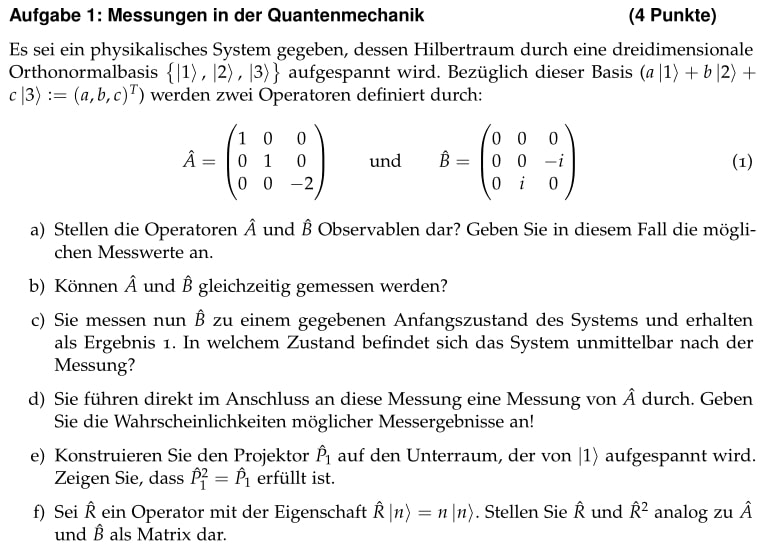
\includegraphics[width=\textwidth]{images/Aufgabe1.jpg}
        \label{fig:1}
    \end{figure}

    \subsection{a)}

    \flushleft{Observable\;}\justifying = Hermitisch:
    \begin{align*}
    A &= A^{\dagger} = \left(A^T\right)^*\\
    B &= B^{\dagger} = \left(A^T\right)^*\\
    A &=
    \begin{pmatrix}
        1 & 0 & 0\\
        0 & 1 & 0\\
        0 & 0 & -2
    \end{pmatrix},\;
    B =
    \begin{pmatrix}
        0 & 0 & 0\\
        0 & 0 & -\text{i}\\
        0 & \text{i} & 0
    \end{pmatrix}\\
    A^{\dagger} &= 
    \begin{pmatrix}
        1 & 0 & 0\\
        0 & 1 & 0\\
        0 & 0 & -2
    \end{pmatrix}^T =
    \begin{pmatrix}
        1 & 0 & 0\\
        0 & 1 & 0\\
        0 & 0 & -2
    \end{pmatrix}^* = A \Rightarrow
    \text{Hermitisch}
    \intertext{\flushleft{Operator\;}\justifying $A$ ist eine Observable.
    }
    B^{\dagger} &= 
    \begin{pmatrix}
        0 & 0 & 0\\
        0 & 0 & \text{i}\\
        0 & -\text{i} & 0
    \end{pmatrix}^T =
    \begin{pmatrix}
        0 & 0 & 0\\
        0 & 0 & -\text{i}\\
        0 & \text{i} & 0
    \end{pmatrix}^* = B \Rightarrow
    \text{Hermitisch}
    \intertext{\flushleft{Operator\;}\justifying $B$ ist eine Observable.
    }
    \intertext{\flushleft{Die\;}\justifying möglichen Messwerte sind die EW der Observablen:
    }
    \text{EW}(A) &= 1\cdot1\cdot(-2)+0-0=-2\\
    \text{EW}(B) &= 0
    \end{align*}

    \subsection{b)}

    \subsection{c)}

    \subsection{d)}

    \subsection{e)}

    \subsection{f)}


\section{Aufgabe 2}

    \begin{figure}[H]
        \centering
        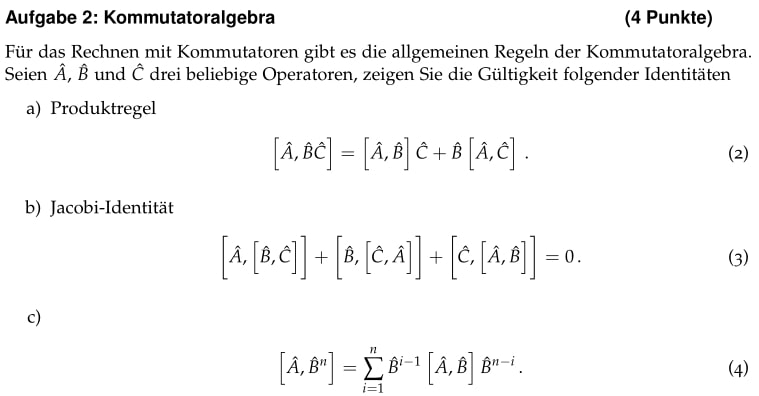
\includegraphics[width=\textwidth]{images/Aufgabe2abc.jpg}
        \label{fig:2}
    \end{figure}

    \begin{figure}[H]
        \centering
        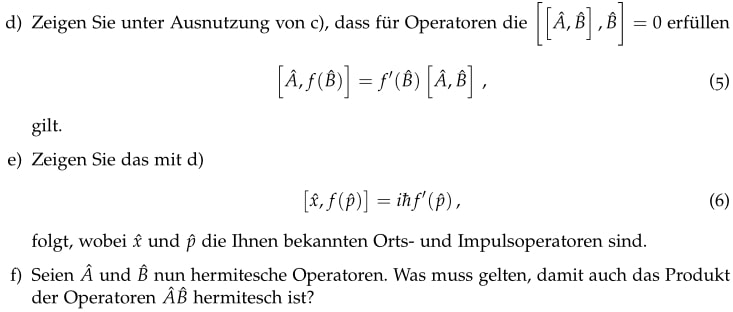
\includegraphics[width=\textwidth]{images/Aufgabe2def.jpg}
        \label{fig:3}
    \end{figure}

    \subsection{a)}
    \begin{align}
    \mathrm{Z\kern-.3em\raise-0.5ex\hbox{Z}} [\hat A, \hat B \hat C] &= [\hat A , \hat B]\hat C + \hat B [\hat A , \hat C]\\
    [hat A , \hat B \hat C] &= \hat A \hat B \hat C - \hat B \hat C \hat A -\hat B \hat A \hat C + \hat B \hat A \hat C\\
    &=(\hat A \hat B - \hat B \hat A) \hat C + \hat B (\hat A \hat C -\hat C \hat A)\\
    &=\underline{\underline{[\hat A , \hat B]\hat C + \hat B [\hat A , \hat C]}}
    \end{align}
    \subsection{b)}
    \begin{align}
    \mathrm{Z\kern-.3em\raise-0.5ex\hbox{Z}} &[\hat A , [\hat B , \hat C]] + [\hat B ,[\hat C, \hat A]]+ [\hat C,[\hat A , \hat B]] =0\\
    [\hat A , [\hat B , \hat C]] &= [\hat A, \hat B \hat C - \hat C \hat B] \\
    &=[\hat A , \hat B \hat C] -[\hat A , \hat C \hat B]\\
    &= \hat A \hat B \hat C -\hat B \hat C \hat A- (\hat A \hat C \hat B-\hat C \hat B \hat A)\\
    [\hat B , [\hat C , \hat A]] &= [\hat B, \hat C \hat A-\hat A \hat C]\\
    &= \hat B \hat C \hat A - \hat C \hat A \hat B - (\hat B \hat A \hat C - \hat A \hat C \hat B)\\
    [\hat C , [\hat A , \hat B]] &= [\hat C , \hat A \hat B]- [\hat C , \hat B \hat A]\\
    &= \hat C \hat A \hat B - \hat A \hat B \hat C -(\hat C \hat B \hat A - \hat B \hat A \hat C)\\
    \Rightarrow &[\hat A , [\hat B , \hat C]] + [\hat B , [\hat C , \hat A]] +[\hat C , [\hat A , \hat B]] = 0
    \end{align}
    \subsection{c)}
    \begin{align}
    \mathrm{Z\kern-.3em\raise-0.5ex\hbox{Z}} [\hat A , \hat B ^n] &= \sum_{i=1}^n \hat B ^{i-1} [\hat A , \hat B ] \hat B ^{n-i}\\
    [\hat A , \hat B ^n] &= [\hat a , \hat B \hat B ^{n-1}]\\
    &= [\hat A , \hat B] \hat B ^{n-1} + \hat B [\hat A , \hat B ^{n-1}]\\
    &= [\hat A , \hat B] \hat B ^{n-1} + \hat B [\hat A , \hat B \hat B ^{n-2}] \\
    &= [\hat A , \hat B] \hat B ^{n-1} + \hat B ([\hat A , \hat B] \hat B ^{n-2} + \hat B [\hat A , \hat B ^ {n-2} ] )\\
    &= [\hat A , \hat B] \hat B ^{n-1} + \hat B [\hat A , \hat B] \hat B ^{n-2} + \hat B ^2 [\hat  A , \hat B ^{n-2}]\\
    &= [\hat A , \hat B] \hat B ^{n-1} + \hat B [\hat A, \hat B] \hat B ^{n-2} + \hdots + \hat B ^{n-1} [\hat A , \hat B]\\
    &=\underline{\underline{ \sum_{i=1}^n \hat B ^{i-1} [\hat A , \hat B] \hat B ^{n-i}}}
    \end{align}
    \subsection{d)}
    \begin{align}
    \mathrm{Z\kern-.3em\raise-0.5ex\hbox{Z}} [\hat A , f8\hat B] &= f'(\hat B) [\hat A , \hat B]\\
    \intertext{
        Potenzriehenansatz für die Funktion f:
    }
    f(\hat B) &= \sum_{n=0}^{\infty} a_n \hat B ^n\\
    f'(\hat B) &= \sum_{n=1}^{\infty} a_n \hat B ^n \\
    [\hat A , \sum_{n=0}^{\infty} a_n \hat B ^n ] &= \sum_{n=0}^{\infty} a_n [\hat A , \hat B ^n]
    \intertext{
        0-tes Summenglied verschwindet und anwenden von c)
    }
    &=\sum_{n=1}^{\infty} a_n \sum_{i=1}^n \hat B ^{i-1} [\hat A , \hat B] \hat B ^{n-i}\\
    \intertext{
        \flushleft{Dadurch}, dass der Kommutator $[[\hat A , \hat B], \hat B]=0$ ist, können die beiden Terme vertauscht werden.
    }
    &=\sum_{n=1}^{\infty} a_n \sum_{i=1}^n \hat B ^{i-1} \hat B ^{n-i} [\hat A , \hat B]\\
    &=\sum_{n=1}^{\infty} a_n \sum_{i=1}^n \hat B^{n-1} [\hat A , \hat B]\\
    &=\sum_{n=1}^{\infty} a_n n \hat B ^{n-1} [\hat A , \hat B]\\
    &= f'(\hat B) [\hat A , \hat B]
    \end{align}
    
    \subsection{e)}
    \begin{align}
    [\hat x , f(\hat p)] &= f' (\hat p ) [\hat x , \hat p] = i \hbar f' (\hat p)
    \end{align}
    \subsection{f)}
    \begin{align}
    \hat A \hat B &= (\hat A \hat B)\\
    &= \hat B ^* \hat A ^*\\
    \Rightarrow & \hat A = \hat B ^* \quad \text{und} \quad \hat B = \hat A ^* 
    \end{align}


\section{Aufgabe 3}

    \begin{figure}[H]
        \centering
        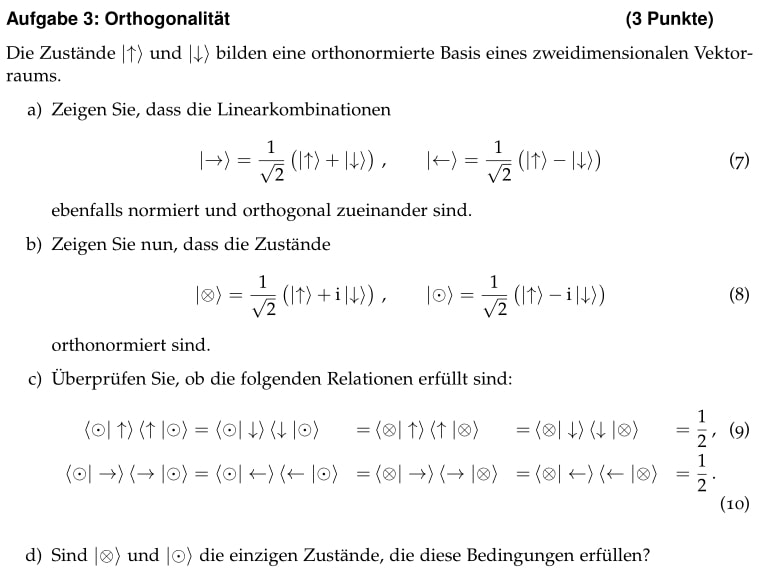
\includegraphics[width=\textwidth]{images/Aufgabe3.jpg}
        \label{fig:4}
    \end{figure}

    \subsection{a)}

    \begin{align*}
        \ket{\to} &= \frac{1}{\sqrt{2}}\left(\ket{\uparrow}+\ket{\downarrow}\right), \qquad \ket{\leftarrow} = \frac{1}{\sqrt{2}}\left(\ket{\uparrow}-\ket{\downarrow}\right)\\
        \Rightarrow\bra{\to} &= \frac{1}{\sqrt{2}}\left(\bra{\uparrow}+\bra{\downarrow}\right), \qquad \bra{\leftarrow} = \frac{1}{\sqrt{2}}\left(\bra{\uparrow}-\bra{\downarrow}\right)
        \intertext{\flushleft{Normierung:\;}\justifying
        }
        \braket{\to} &= \left( \frac{1}{\sqrt{2}}\left(\bra{\uparrow}+\bra{\downarrow}\right) \right) \left(  \frac{1}{\sqrt{2}}\left(\ket{\uparrow}+\ket{\downarrow}\right) \right)\\
        &= \frac{1}{2} \underbrace{\braket{\uparrow}}_{=1} + \frac{1}{2} \underbrace{\braket{\uparrow}{\downarrow}}_{=0}
        + \frac{1}{2} \underbrace{\braket{\downarrow}{\uparrow}}_{=0} + \frac{1}{2} \underbrace{\braket{\downarrow}{\downarrow}}_{=1}\\
        &= \frac{1}{2}+\frac{1}{2} = 1\\
        \\
        \braket{\leftarrow} &= \left( \frac{1}{\sqrt{2}}\left(\bra{\uparrow}-\bra{\downarrow}\right) \right) \left(  \frac{1}{\sqrt{2}}\left(\ket{\uparrow}-\ket{\downarrow}\right) \right)\\
        &= \frac{1}{2} \underbrace{\braket{\uparrow}}_{=1} - \frac{1}{2} \underbrace{\braket{\uparrow}{\downarrow}}_{=0}
        - \frac{1}{2} \underbrace{\braket{\downarrow}{\uparrow}}_{=0} + \frac{1}{2} \underbrace{\braket{\downarrow}{\downarrow}}_{=1}\\
        &= \frac{1}{2}+\frac{1}{2} = 1
        \intertext{\flushleft{Orthogonalität:\;}\justifying
        }
        \braket{\leftarrow}{\to} &= \left( \frac{1}{\sqrt{2}}\left(\bra{\uparrow}-\bra{\downarrow}\right) \right) \left(  \frac{1}{\sqrt{2}}\left(\ket{\uparrow}+\ket{\downarrow}\right) \right)\\
        &= \frac{1}{2} \underbrace{\braket{\uparrow}}_{=1} + \frac{1}{2} \underbrace{\braket{\uparrow}{\downarrow}}_{=0}
        - \frac{1}{2} \underbrace{\braket{\downarrow}{\uparrow}}_{=0} - \frac{1}{2} \underbrace{\braket{\downarrow}{\downarrow}}_{=1}\\
        &= \frac{1}{2}-\frac{1}{2} = 0
    \end{align*}

    \subsection{b)}

    \begin{align*}
        \ket{\otimes} &= \frac{1}{\sqrt{2}}\left(\ket{\uparrow}+\text{i}\ket{\downarrow}\right), \qquad \ket{\odot} = \frac{1}{\sqrt{2}}\left(\ket{\uparrow}-\text{i}\ket{\downarrow}\right)\\
        \Rightarrow\bra{\otimes} &= \frac{1}{\sqrt{2}}\left(\bra{\uparrow}-\bra{\downarrow}\text{i}\right), \qquad \bra{\odot} = \frac{1}{\sqrt{2}}\left(\bra{\uparrow}+\bra{\downarrow}\text{i}\right)
        \intertext{\flushleft{Normierung:\;}\justifying
        }
        \braket{\otimes} &= \left( \frac{1}{\sqrt{2}}\left(\bra{\uparrow}-\bra{\downarrow}\text{i}\right) \right) \left(  \frac{1}{\sqrt{2}}\left(\ket{\uparrow}+\text{i}\ket{\downarrow}\right) \right)\\
        &= \frac{1}{2} \underbrace{\braket{\uparrow}}_{=1} + \frac{\text{i}}{2} \underbrace{\braket{\uparrow}{\downarrow}}_{=0}
        - \frac{\text{i}}{2} \underbrace{\braket{\downarrow}{\uparrow}}_{=0} - \frac{\text{i}^2}{2} \underbrace{\braket{\downarrow}{\downarrow}}_{=1}\\
        &= \frac{1}{2}-\frac{\text{i}^2}{2} = 1\\
        \braket{\odot} &= \left( \frac{1}{\sqrt{2}}\left(\bra{\uparrow}+\bra{\downarrow}\text{i}\right) \right) \left(  \frac{1}{\sqrt{2}}\left(\ket{\uparrow}-\text{i}\ket{\downarrow}\right) \right)\\
        &= \frac{1}{2} \underbrace{\braket{\uparrow}}_{=1} - \frac{\text{i}}{2} \underbrace{\braket{\uparrow}{\downarrow}}_{=0}
        + \frac{\text{i}}{2} \underbrace{\braket{\downarrow}{\uparrow}}_{=0} - \frac{\text{i}^2}{2} \underbrace{\braket{\downarrow}{\downarrow}}_{=1}\\
        &= \frac{1}{2}-\frac{\text{i}^2}{2} = 1
        \intertext{\flushleft{Orthogonalität:\;}\justifying
        }
        \braket{\otimes}{\odot} &= \left( \frac{1}{\sqrt{2}}\left(\bra{\uparrow}-\bra{\downarrow}\text{i}\right) \right) \left(  \frac{1}{\sqrt{2}}\left(\ket{\uparrow}-\text{i}\ket{\downarrow}\right) \right)\\
        &= \frac{1}{2} \underbrace{\braket{\uparrow}}_{=1} - \frac{\text{i}}{2} \underbrace{\braket{\uparrow}{\downarrow}}_{=0}
        - \frac{\text{i}}{2} \underbrace{\braket{\downarrow}{\uparrow}}_{=0} + \frac{\text{i}^2}{2} \underbrace{\braket{\downarrow}{\downarrow}}_{=1}\\
        &= \frac{1}{2}+\frac{\text{i}^2}{2} = 0
    \end{align*}

    \subsection{c)}

    \begin{align*}
    \braket{\odot}{\uparrow}\braket{\uparrow}{\odot} &= 
    \left( \frac{1}{\sqrt{2}} \underbrace{\braket{\uparrow}{\uparrow}}_{=1} + \frac{\text{i}}{\sqrt{2}} \underbrace{\braket{\downarrow}{\uparrow}}_{=0} \right)
    \left( \frac{1}{\sqrt{2}} \underbrace{\braket{\uparrow}{\uparrow}}_{=1} - \frac{\text{i}}{\sqrt{2}} \underbrace{\braket{\uparrow}{\downarrow}}_{=0} \right)\\
    &= \frac{1}{\sqrt{2}} \cdot \frac{1}{\sqrt{2}} = \frac{1}{2}\\
    \braket{\odot}{\downarrow}\braket{\downarrow}{\odot} &= 
    \left( \frac{1}{\sqrt{2}} \underbrace{\braket{\uparrow}{\downarrow}}_{=0} + \frac{\text{i}}{\sqrt{2}} \underbrace{\braket{\downarrow}{\downarrow}}_{=1} \right)
    \left( \frac{1}{\sqrt{2}} \underbrace{\braket{\downarrow}{\uparrow}}_{=0} - \frac{\text{i}}{\sqrt{2}} \underbrace{\braket{\downarrow}{\downarrow}}_{=1} \right)\\
    &= \frac{i}{\sqrt{2}} \cdot \frac{(-i)}{\sqrt{2}} = \frac{1}{2}\\
    \braket{\otimes}{\uparrow}\braket{\uparrow}{\otimes} &= 
    \left( \frac{1}{\sqrt{2}} \underbrace{\braket{\uparrow}{\uparrow}}_{=1} - \frac{\text{i}}{\sqrt{2}} \underbrace{\braket{\downarrow}{\uparrow}}_{=0} \right)
    \left( \frac{1}{\sqrt{2}} \underbrace{\braket{\uparrow}{\uparrow}}_{=1} + \frac{\text{i}}{\sqrt{2}} \underbrace{\braket{\uparrow}{\downarrow}}_{=0} \right)\\
    &= \frac{1}{\sqrt{2}} \cdot \frac{1}{\sqrt{2}} = \frac{1}{2}\\
    \braket{\otimes}{\downarrow}\braket{\downarrow}{\otimes} &= 
    \left( \frac{1}{\sqrt{2}} \underbrace{\braket{\uparrow}{\downarrow}}_{=0} - \frac{\text{i}}{\sqrt{2}} \underbrace{\braket{\downarrow}{\downarrow}}_{=1} \right)
    \left( \frac{1}{\sqrt{2}} \underbrace{\braket{\downarrow}{\uparrow}}_{=0} + \frac{\text{i}}{\sqrt{2}} \underbrace{\braket{\downarrow}{\downarrow}}_{=1} \right)\\
    &= \frac{-i}{\sqrt{2}} \cdot \frac{i}{\sqrt{2}} = \frac{1}{2}\\
    \end{align*}

    \flushleft{Die\;}\justifying $[...]$-Klammern sind hier keine Kommutatorklammern!
    \begin{align*}
        \braket{\odot}{\to}\braket{\to}{\odot} &=
    \left[ \left( \frac{1}{\sqrt{2}}\left(\bra{\uparrow}+\bra{\downarrow}\text{i}\right) \right) 
    \left( \frac{1}{\sqrt{2}}\left(\ket{\uparrow}+\ket{\downarrow}\right) \right) \right] 
    \left[ \left( \frac{1}{\sqrt{2}}\left(\bra{\uparrow}+\bra{\downarrow}\right) \right) 
    \left( \frac{1}{\sqrt{2}}\left(\ket{\uparrow}-\text{i}\ket{\downarrow}\right) \right) \right]\\
    &= \left( \frac{1}{2} \underbrace{\braket{\uparrow}{\uparrow}}_{=1} 
    + \frac{1}{2} \underbrace{\braket{\uparrow}{\downarrow}}_{=0}
    + \frac{\text{i}}{2} \underbrace{\braket{\downarrow}{\uparrow}}_{=0} 
    + \frac{\text{i}}{2} \underbrace{\braket{\downarrow}{\downarrow}}_{=1} \right)
    \left( \frac{1}{2} \underbrace{\braket{\uparrow}{\uparrow}}_{=1} 
    - \frac{\text{i}}{2} \underbrace{\braket{\uparrow}{\downarrow}}_{=0}
    + \frac{1}{2} \underbrace{\braket{\downarrow}{\uparrow}}_{=0} 
    - \frac{\text{i}}{2} \underbrace{\braket{\downarrow}{\downarrow}}_{=1} \right)\\
    &= \left( \frac{1}{2} + \frac{\text{i}}{2} \right) \left( \frac{1}{2} - \frac{\text{i}}{2} \right)\\
    &= \frac{1}{4} - \frac{\text{i}}{4} + \frac{1}{4} + \frac{\text{i}}{4} = \frac{1}{2}\\
        \braket{\odot}{\leftarrow}\braket{\leftarrow}{\odot} &=
    \left[ \left( \frac{1}{\sqrt{2}}\left(\bra{\uparrow}+\bra{\downarrow}\text{i}\right) \right) 
    \left( \frac{1}{\sqrt{2}}\left(\ket{\uparrow}-\ket{\downarrow}\right) \right) \right] 
    \left[ \left( \frac{1}{\sqrt{2}}\left(\bra{\uparrow}-\bra{\downarrow}\right) \right) 
    \left( \frac{1}{\sqrt{2}}\left(\ket{\uparrow}-\text{i}\ket{\downarrow}\right) \right) \right]\\
    &= \left( \frac{1}{2} \underbrace{\braket{\uparrow}{\uparrow}}_{=1} 
    - \frac{1}{2} \underbrace{\braket{\uparrow}{\downarrow}}_{=0}
    + \frac{\text{i}}{2} \underbrace{\braket{\downarrow}{\uparrow}}_{=0} 
    - \frac{\text{i}}{2} \underbrace{\braket{\downarrow}{\downarrow}}_{=1} \right)
    \left( \frac{1}{2} \underbrace{\braket{\uparrow}{\uparrow}}_{=1} 
    - \frac{\text{i}}{2} \underbrace{\braket{\uparrow}{\downarrow}}_{=0}
    - \frac{1}{2} \underbrace{\braket{\downarrow}{\uparrow}}_{=0} 
    + \frac{\text{i}}{2} \underbrace{\braket{\downarrow}{\downarrow}}_{=1} \right)\\
    &= \left( \frac{1}{2} - \frac{\text{i}}{2} \right) \left( \frac{1}{2} + \frac{\text{i}}{2} \right)\\
    &= \frac{1}{4} + \frac{\text{i}}{4} - \frac{1}{4} + \frac{\text{i}}{4} = \frac{1}{2}\\
        \braket{\otimes}{\to}\braket{\to}{\otimes} &=
    \left[ \left( \frac{1}{\sqrt{2}}\left(\bra{\uparrow}-\bra{\downarrow}\text{i}\right) \right) 
    \left( \frac{1}{\sqrt{2}}\left(\ket{\uparrow}+\ket{\downarrow}\right) \right) \right] 
    \left[ \left( \frac{1}{\sqrt{2}}\left(\bra{\uparrow}+\bra{\downarrow}\right) \right) 
    \left( \frac{1}{\sqrt{2}}\left(\ket{\uparrow}+\text{i}\ket{\downarrow}\right) \right) \right]\\
    &= \left( \frac{1}{2} \underbrace{\braket{\uparrow}{\uparrow}}_{=1} 
    + \frac{1}{2} \underbrace{\braket{\uparrow}{\downarrow}}_{=0}
    - \frac{\text{i}}{2} \underbrace{\braket{\downarrow}{\uparrow}}_{=0} 
    - \frac{\text{i}}{2} \underbrace{\braket{\downarrow}{\downarrow}}_{=1} \right)
    \left( \frac{1}{2} \underbrace{\braket{\uparrow}{\uparrow}}_{=1} 
    + \frac{\text{i}}{2} \underbrace{\braket{\uparrow}{\downarrow}}_{=0}
    + \frac{1}{2} \underbrace{\braket{\downarrow}{\uparrow}}_{=0} 
    + \frac{\text{i}}{2} \underbrace{\braket{\downarrow}{\downarrow}}_{=1} \right)\\
    &= \left( \frac{1}{2} - \frac{\text{i}}{2} \right) \left( \frac{1}{2} + \frac{\text{i}}{2} \right)\\
    &= \frac{1}{4} + \frac{\text{i}}{4} - \frac{1}{4} + \frac{\text{i}}{4} = \frac{1}{2}\\
        \braket{\otimes}{\leftarrow}\braket{\leftarrow}{\otimes} &=
    \left[ \left( \frac{1}{\sqrt{2}}\left(\bra{\uparrow}-\bra{\downarrow}\text{i}\right) \right) 
    \left( \frac{1}{\sqrt{2}}\left(\ket{\uparrow}-\ket{\downarrow}\right) \right) \right] 
    \left[ \left( \frac{1}{\sqrt{2}}\left(\bra{\uparrow}-\bra{\downarrow}\right) \right) 
    \left( \frac{1}{\sqrt{2}}\left(\ket{\uparrow}+\text{i}\ket{\downarrow}\right) \right) \right]\\
    &= \left( \frac{1}{2} \underbrace{\braket{\uparrow}{\uparrow}}_{=1} 
    - \frac{1}{2} \underbrace{\braket{\uparrow}{\downarrow}}_{=0}
    - \frac{\text{i}}{2} \underbrace{\braket{\downarrow}{\uparrow}}_{=0} 
    + \frac{\text{i}}{2} \underbrace{\braket{\downarrow}{\downarrow}}_{=1} \right)
    \left( \frac{1}{2} \underbrace{\braket{\uparrow}{\uparrow}}_{=1} 
    + \frac{\text{i}}{2} \underbrace{\braket{\uparrow}{\downarrow}}_{=0}
    - \frac{1}{2} \underbrace{\braket{\downarrow}{\uparrow}}_{=0} 
    - \frac{\text{i}}{2} \underbrace{\braket{\downarrow}{\downarrow}}_{=1} \right)\\
    &= \left( \frac{1}{2} + \frac{\text{i}}{2} \right) \left( \frac{1}{2} - \frac{\text{i}}{2} \right)\\
    &= \frac{1}{4} - \frac{\text{i}}{4} + \frac{1}{4} + \frac{\text{i}}{4} = \frac{1}{2}
    \end{align*}

    \subsection{d)}


\section{Aufgabe 4}

    \begin{figure}[H]
        \centering
        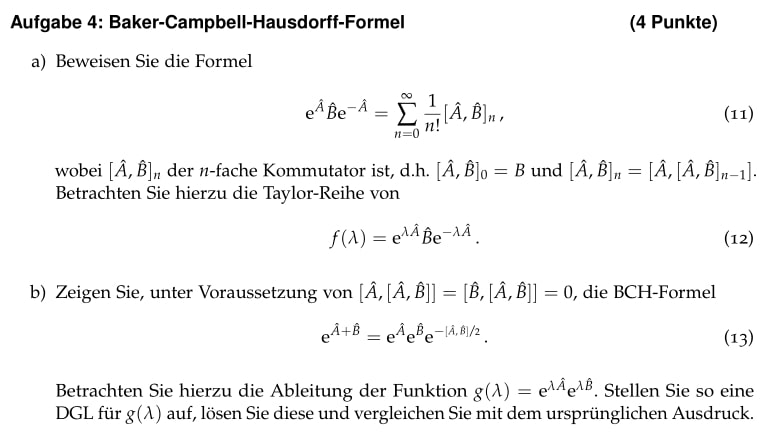
\includegraphics[width=\textwidth]{images/Aufgabe4.jpg}
        \label{fig:5}
    \end{figure}

    \subsection{a)}
    \begin{align}
    \mathrm{Z\kern-.3em\raise-0.5ex\hbox{Z}} e^{\hat A} \hat B e^{-\hat A} &= \sum_{n=0}^{\infty} \frac{1}{n!} [\hat A , \hat B]_n\\
    f(\lambda) &= e^{\lambda \hat A} \hat B e^{- \lambda \hat A}\\
    &= e^{\lambda \hat A} [\hat A , \hat B]_0 e^{-\lambda \hat A}\\
    \intertext{
        Entwicklung von f in eine Taylorreihe um 0
    }
    f'(\lambda) &= e^{\lambda \hat A} (\hat A \hat B - \hat B \hat A) e^{-\lambda \hat A}\\
    &=e{\lambda \hat A} [\hat A , \hat B]_1 e^{-\lambda \hat A}\\
    f''{\lambda} &= e^{\lambda \hat A} (\hat A [\hat A, \hat B]_1-[\hat A , \hat B]_1 \hat A) e^{-\lambda \hat A}\\
    &= e^{\lambda \hat A} [\hat A , [\hat A,\hat B]_1] e^{-\lambda \hat A}\\
    &=  e^{\lambda \hat A} [\hat A , \hat B]_2 e^{-\lambda \hat A}\\
    \intertext{
        Induktion:
    }
    \mathrm{Z\kern-.3em\raise-0.5ex\hbox{Z}} f^{(n)} &= e^{\lambda \hat A} [\hat A , \hat B]_n e^{-\lambda \hat A}\\
    \intertext{
        Induktionsanfang
    }
    n &=0\\
    f^{(0)} &=e^{\lambda \hat A} [\hat A , \hat B]_0 e^{-\lambda \hat A} \surd
    \intertext{
        Induktionsvorraussetzung
    }
    f^{(n)} &= e^{\lambda \hat A} [\hat A , \hat B]_n e^{-\lambda \hat A}\\
    \intertext{gilt für ein $n \in \symbb{N} $}
    [\hat A , \hat B]_n &= [\hat A , [\hat A , \hat B]_{n-1} ]
    \intertext{
        Induktionsbehauptung
    }
    n &\to n+1\\
    \frac{\partial}{\partial \lambda} f^{(n)} &= \frac{\partial}{\partial \lambda} (e^{\lambda \hat A} [\hat A ,\hat B]_n e^{-\lambda \hat A} )\\
    f^{(n+1)} &= e^{\lambda \hat A} (\hat A [\hat A , \hat B]_n-[\hat A , \hat B]_n \hat A) e^{-\lambda \hat A} \\
    &= e^{\lambda \hat A} [\hat A ,[\hat A, \hat B]_n] e^{-\lambda \hat A} \\
    f^{(n+1)} &= e^{\lambda \hat A} [\hat A , \hat B]_{n+1} e^{-\lambda \hat A} \surd\\
    \intertext{
        Aufstellen der Taylorreihe
    }
    f^{(n)}(0) &= [\hat A , \hat B]_n \\
    \Rightarrow T(\lambda , 0)&= \sum_{n=0}^{\infty} \frac{1}{n!} [\hat A , \hat B] \lambda ^n\\
    T(1,0)&= \sum_{n=0}^{\infty} \frac{1}{n!} [\hat A , \hat B]_n \\
    f(1) &= e^{\hat A} \hat B e^{-\hat A}\\
    \Rightarrow e^{\hat A} \hat B e^{-\hat A} &= \sum_{n=0}^{\infty} \frac{1}{n!} [\hat A , \hat B]_n
    \end{align}
    \subsection{b)}
    \begin{align}
    \mathrm{Z\kern-.3em\raise-0.5ex\hbox{Z}} e^{\hat A + \hat B} &= e^{\hat A} e^{\hat B} e^{-[\hat A ,\hat B]/2}\\
    e^{\lambda \hat A} \hat B e^{-\lambda \hat A} &= \sum_{n=0}^{\infty} \frac{1}{n!} [\hat A , \hat B]_n \lambda ^n\\
    &=\sum_{n=0}^{\infty} \frac{1}{n!} [\hat A ,[\hat A , \hat B]_{n-1}] \lambda ^n\\
    \intertext{
        Aufgrund der Bedingung $[\hat A ,[\hat A, \hat B]] =0 $ werden alle Summanenglieder
        außer für $n=0$ und $n=1$ 0.
    }
    \Rightarrow &= \frac{1}{0!} \hat B + \frac{1}{1!} [\hat A , \hat B] \lambda\\
    e^{\lambda \hat A} \hat B e^{-\lambda \hat A } &= \hat B + \lambda [\hat A , \hat B]\\
    e^{\lambda \hat A} \hat B &=(\hat B + \lambda [\hat A, \hat B])e^{\lambda \hat A}\\
    \frac{\dif{}}{\dif{\lambda}} (e^{\lambda \hat A} e^{\lambda \hat B}) &= \hat A e^{\lambda \hat A} e^{\lambda \hat B} + e^{\lambda \hat A} \hat B e^{\lambda \hat B}\\
    &= \hat A e^{\lambda \hat A} e^{\lambda \hat B} + (\hat B + \lambda[\hat A , \hat B])e^{\lambda \hat A} e^{\lambda \hat B}\\
    \frac{\dif{g(\lambda)}}{\dif{\lambda}}&= (\hat A + \hat B + \lambda[\hat A, \hat B])g(\lambda)\\
    \intertext{
        Allgemeine Lösung der DGL lautet
    }
    g(\lambda) &= C \exp\left(\int \hat A + \hat B + \lambda [\hat A , \hat B]\,\dif{\lambda} \right)\\
    &= C \exp(\hat A \lambda + \hat B \lambda + \frac{1}{2} \lambda ^2 [\hat A , \hat B])
    \intertext{
        Vergleich der DGL-Lösung mit der ursprünglichen Funktion g
    }
    e^{\lambda \hat A} e^{\lambda \hat B} &= C e^{\hat A \lambda + \hat B \lambda + \frac{1}{2} \lambda ^2 [\hat A , \hat B]}
    \intertext{
        Wähle $C=1$ und $\lambda = 1$ 
    }
    e^{\hat A} e^{\hat B} &= e^{\hat A + \hat B  + \frac{1}{2} [\hat A , \hat B]}
    \intertext{
        Da $[\hat A , \hat B] $ mit $\hat B$ und $\hat A$ kommutiert, lässt sich die rechte Seite 
    folgendermaßen schreibn
    }
    &=e^{\hat A + \hat B} e^{\frac{1}{2}[\hat A , \hat B]}\\
    e^{\hat A + \hat B} &= e^{\hat A} e^{\hat B} e^{-\frac{1}{2} [\hat A , \hat B]}
    \end{align}


\end{document}